\documentclass[11pt]{article}
\usepackage{amsmath, amssymb, amsfonts, amsthm}
\usepackage{geometry}
\geometry{letterpaper, margin=0.5in}
\usepackage{booktabs}
\usepackage{tikz}
\usepackage{hyperref}
\usepackage{makecell}

\newcommand{\noi}{\noindent}

\theoremstyle{definition} 
\newtheorem{definition}{Definition}[section]

\newif\ifrootsystemirreducible
\rootsystemirreducibletrue

\title{Pinned group summary: SO(n=5, q=1)}
\author{Pinning-Sympy automated output}
\date{\today}

\begin{document}

\maketitle
\tableofcontents

\newpage

\section{Basic group attributes}

\begin{tabular}{|l|l|}
	\hline
    Group & SO(n=5, q=1) \\
	\hline
    Matrix size & $5 \times 5$ \\
	\hline
    Rank & $1$ \\
	\hline
	Defining equations & $DefiningEquationPlaceholder$ \\
	\hline
\end{tabular}

\subsection{Symmetric bilinear form}
\begin{tabular}{|l|l|}
    \hline
    Dimension & 5 \\
    \hline
    Witt index & 1 \\
    \hline
    Primitive element & N/A \\
    \hline
    Epsilon & N/A \\
    \hline
\end{tabular}

\bigskip
\noindent Matrix: \(
\left[\begin{matrix}0 & 1 & 0 & 0 & 0\\1 & 0 & 0 & 0 & 0\\0 & 0 & c_{0} & 0 & 0\\0 & 0 & 0 & c_{1} & 0\\0 & 0 & 0 & 0 & c_{2}\end{matrix}\right]
\)



\subsection{Lie algebra}

The defining equations for the Lie algebra are:
\[
LieAlgebraEquationPlaceholder
\]
A generic element of the Lie algebra is:
\[
\left[\begin{matrix}x_{0 0} & 0 & - c_{0} x_{2 1} & - c_{1} x_{3 1} & - c_{2} x_{4 1}\\0 & - x_{0 0} & - c_{0} x_{2 0} & - c_{1} x_{3 0} & - c_{2} x_{4 0}\\x_{2 0} & x_{2 1} & 0 & x_{2 3} & x_{2 4}\\x_{3 0} & x_{3 1} & - \frac{c_{0} x_{2 3}}{c_{1}} & 0 & x_{3 4}\\x_{4 0} & x_{4 1} & - \frac{c_{0} x_{2 4}}{c_{2}} & - \frac{c_{1} x_{3 4}}{c_{2}} & 0\end{matrix}\right]
\]

\subsection{Torus}

The torus has rank $1$. A generic element of the torus is
\[
\left[\begin{matrix}t_{0} & 0 & 0 & 0 & 0\\0 & \frac{1}{t_{0}} & 0 & 0 & 0\\0 & 0 & 1 & 0 & 0\\0 & 0 & 0 & 1 & 0\\0 & 0 & 0 & 0 & 1\end{matrix}\right]
\]
The rows of the matrix below are trivial characters:
\[
\left[\begin{matrix}1 & 1 & 0 & 0 & 0\\1 & 1 & 1 & 1 & 1\end{matrix}\right]
\]

\newpage
\section{Root system}

\begin{tabular}{|l|l|}
	\hline
    Dynkin type & $A_1$ \\
	\hline
    Irreducible & True \\
	\hline
    Reduced & True \\
	\hline
	Simply laced & True \\
	\hline
	Number of roots & $2$ \\
	\hline
\end{tabular}

\subsection{Dynkin diagram}

\ifrootsystemirreducible
The root system is irreducible and has Dynkin diagram:
\else
The root system is reducible with RootSystemComponentsPlaceholder components. The Dynkin diagrams of the respective components are:
\fi

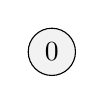
\begin{tikzpicture}[
    node/.style={circle, draw, fill=black!5, minimum size=6mm, inner sep=0pt},
    arrow/.style={-latex, thick},
    doublearrow/.style={double, double distance=2pt, -latex, thick},
    triplearrow/.style={double, double distance=4pt, -latex, thick},
    plain/.style={thick},
    baseline=(current bounding box.center)
]
    \node[node] (0) at (0.00, 0.00) {$0$};
\end{tikzpicture}

\subsection{Cartan matrix}

\ifrootsystemirreducible
The root system is irreducible and has Cartan matrix:
\else
The root system is reducible with RootSystemComponentsPlaceholder components. The Cartan matrices of the respective components are:
\fi

\[
\left[\begin{matrix}2\end{matrix}\right]
\]

\subsection{Roots}

\begin{tabular}{|l|c|c|c|}
    \hline
    \textbf{Root} & \textbf{Simple} & \textbf{Sign} & \textbf{Multipliable} \\
    \hline
    $\left( -1, \  0, \  0, \  0, \  0\right)$ & No & $-$ & No \\
    \hline
    $\left( 1, \  0, \  0, \  0, \  0\right)$ & Yes & $+$ & No \\
    \hline
\end{tabular}


\subsection{Coroots}

\begin{tabular}{|l|l|}
    \hline
    \textbf{Root} & \textbf{Coroot} \\
    \hline
    $\left( -1, \  0, \  0, \  0, \  0\right)$ & $\left( -2, \  2, \  0, \  0, \  0\right)$ \\
    \hline
    $\left( 1, \  0, \  0, \  0, \  0\right)$ & $\left( 2, \  -2, \  0, \  0, \  0\right)$ \\
    \hline
\end{tabular}


\subsection{Linear combinations of roots}

\begin{definition}
For two roots $\alpha, \beta$ in a root system $\Phi$, the set of positive integral linear combinations of $\alpha, \beta$ that are also roots is denoted
\(
	(\alpha, \beta) = \{ i \alpha + j \beta \in \Phi : i, j \in \mathbb{Z}_{\ge 1} \}
\).
\end{definition}

\noindent No pairs of roots generate positive integer linear combinations.


\newpage
\section{Root spaces}

\subsection{Dimensions}

The table below lists each root along with the dimension of the associated root space (and root subgroup).

\bigskip

\noindent \begin{tabular}{|l|c|}
    \hline
    \textbf{Root ($\alpha$)} & \textbf{Dimension of root space ($d_{\alpha}$)} \\
    \hline
    $\left( -1, \  0, \  0, \  0, \  0\right)$ & 3 \\
    \hline
    $\left( 1, \  0, \  0, \  0, \  0\right)$ & 3 \\
    \hline
\end{tabular}


\subsection{Root space table}

\noi The table below lists each root along with a generic element of the associated root space (inside the Lie algebra). Include a definition here? INCOMPLETE

\bigskip

\noindent \begin{tabular}{|l|c|}
    \hline
    \textbf{Root ($\alpha$)} & \textbf{Generic element of root space} \\
    \hline
    $\left( -1, \  0, \  0, \  0, \  0\right)$ & $\left[\begin{matrix}0 & 0 & 0 & 0 & 0\\0 & 0 & - c_{0} u_{2} & - c_{1} u_{0} & - c_{2} u_{1}\\u_{2} & 0 & 0 & 0 & 0\\u_{0} & 0 & 0 & 0 & 0\\u_{1} & 0 & 0 & 0 & 0\end{matrix}\right]$ \\
    \hline
    $\left( 1, \  0, \  0, \  0, \  0\right)$ & $\left[\begin{matrix}0 & 0 & - c_{0} u_{1} & - c_{1} u_{0} & - c_{2} u_{2}\\0 & 0 & 0 & 0 & 0\\0 & u_{1} & 0 & 0 & 0\\0 & u_{0} & 0 & 0 & 0\\0 & u_{2} & 0 & 0 & 0\end{matrix}\right]$ \\
    \hline
\end{tabular}


\newpage
\section{Root subgroups}

\subsection{Root subgroup table}

\noi The table below lists each root along with a generic element of the associated root subgroup.

\bigskip

\noindent \begin{tabular}{|l|c|}
    \hline
    \textbf{Root ($\alpha$)} & \textbf{Generic element of root space} \\
    \hline
    $\left( -1, \  0, \  0, \  0, \  0\right)$ & $\left[\begin{matrix}1 & 0 & 0 & 0 & 0\\- \frac{c_{0} u_{2}^{2}}{2} - \frac{c_{1} u_{0}^{2}}{2} - \frac{c_{2} u_{1}^{2}}{2} & 1 & - c_{0} u_{2} & - c_{1} u_{0} & - c_{2} u_{1}\\u_{2} & 0 & 1 & 0 & 0\\u_{0} & 0 & 0 & 1 & 0\\u_{1} & 0 & 0 & 0 & 1\end{matrix}\right]$ \\
    \hline
    $\left( 1, \  0, \  0, \  0, \  0\right)$ & $\left[\begin{matrix}1 & - \frac{c_{0} u_{1}^{2}}{2} - \frac{c_{1} u_{0}^{2}}{2} - \frac{c_{2} u_{2}^{2}}{2} & - c_{0} u_{1} & - c_{1} u_{0} & - c_{2} u_{2}\\0 & 1 & 0 & 0 & 0\\0 & u_{1} & 1 & 0 & 0\\0 & u_{0} & 0 & 1 & 0\\0 & u_{2} & 0 & 0 & 1\end{matrix}\right]$ \\
    \hline
\end{tabular}


\subsection{Homomorphism property}

\noi Background theoretical info on homomorphism/pseudo-homomorphism property INCOMPLETE

\bigskip

HomomorphismDefectTablePlaceholder

\noi Below is an explicit formulation of the homomorphism/pseudo-homomorphism identities.

\bigskip

HomomorphismDefectIdentitiesPlaceholder

\newpage
\section{Commutators}

\noi Background theoretical info on commutator relation INCOMPLETE

\noi Because of its relevance to commutators, we repeat here the table of linear combinations of roots.

\noindent No pairs of roots generate positive integer linear combinations.


\subsection{Commutator coefficient table}

\noi The table below gives the coefficients $N_{ij}^{\alpha\beta}$.

CommutatorCoefficientTablePlaceholder

\subsection{Commutator identities}

\noi Below is an explicit formulation of the commutator formula identities.

CommutatorIdentitiesPlaceholder

\newpage
\section{Weyl group}

\noi Background theoretical info on Weyl group, especially as realized inside the group, including info on conjugation between root subgroups INCOMPLETE

\subsection{Weyl group elements}

\noi The table below lists roots along with an associated Weyl group element.

WeylGroupPlaceholder

\subsection{Weyl group conjugation coefficients}

\noi The table below lists roots along with the coefficients obtain in performing conjugation by an associated Weyl element.

WeylConjugationCoefficientPlaceholder

\subsection{Weyl group conjugation identities}

\noi Below is an explicit formulation of the Weyl group conjugation identities.

WeylConjugationIdentitiesPlaceholder

\end{document}